\paragraph*{}
  Comme dit plus tôt, pour pouvoir passer de l'équation de Boltzmann aux LBM\footnote{Pour plus de précisions vous pouvez 
  lire l'article \cite{PhysRevE.56.6811}.} il faut discrétiser l'espace des phases.
  Dans le volume d'abord : $\r$ est borné à notre espace d'intérêt et on échantillonne cet espace avec un pas de longueur 
  $\dl$.
  Puis l'on vas échantillonner nos vitesses dans notre cas on veux que pour chaque instant $\dt$ des particules puissent 
  s'échanger avec les deux plus proches voisins d'un nœud de notre réseau.
  Afin de préserver l'isotropie des vitesses $\v$ nous ne privilégierons aucune direction en échantillonnant de la sorte
  on obtiens le jeu de vitesses représenté sur la figure \ref{fig:ei}.

  \begin{figure}[htp]
    \centering
    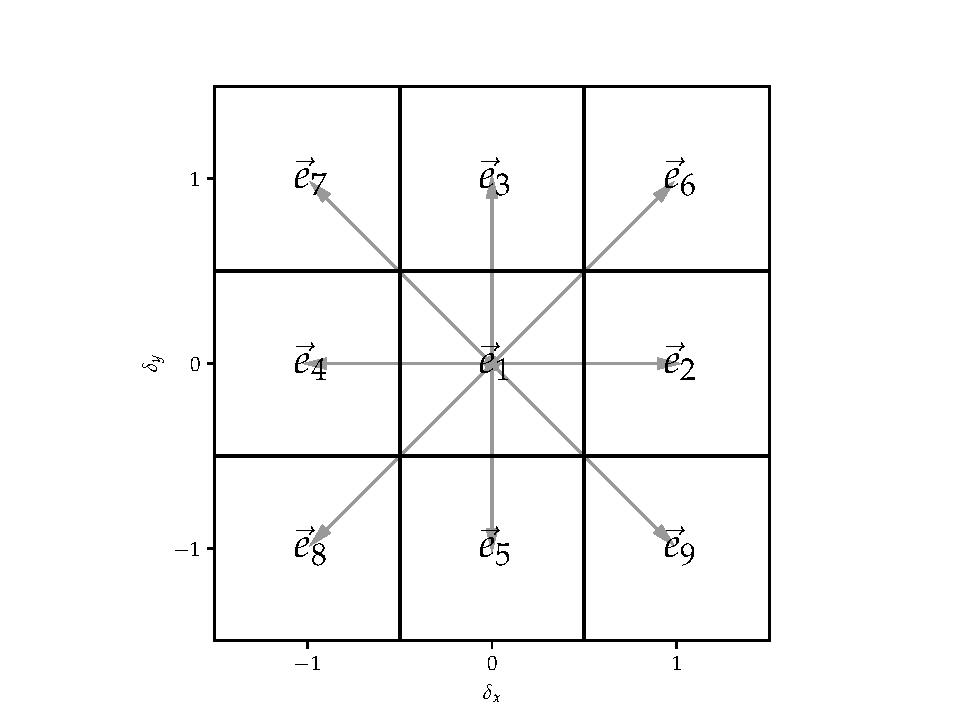
\includegraphics[width=\linewidth]{ei.pdf}
    \caption{Vitesses $\ei$ du réseau pour D2Q9.}
    \label{fig:ei}
  \end{figure}
  
  Il faut bien comprendre que nous aurions pu définir n'importe quel jeu de vitesses $\ei$ arbitraire\footnote{À partir du   
  moment où l'on respecte l'isotropie.}, tout comme on as choisi un jeu de positions $\r$ dans lequel notre simulation ce 
  déroulera, cette discrétisation dans l'espace des phases n'est fondamentalement pas beaucoup différent de ce que l'on
  fait plus couramment.
  
  Étant donnée la construction de notre réseau on peux définir la vitesse de maille $c$ :
  \begin{equation} \label{eq:c}
    c := \frac{\dl}{\dt}.
  \end{equation}
  
  A l'aide de la figure \ref{fig:ei} et de la définition de $c$ on peux définir les valeurs de $\ei$ pour notre 
  simulation:
  
  \begin{equation}
    \ei := c
    \begin{bmatrix}
      0&1&0&-1&0&1&-1&-1&1\\
      0&0&1&0&-1&1&1&-1&-1
    \end{bmatrix}.
  \end{equation}

  En utilisant la distribution de Maxwell-Boltzmann il nous est possible de calculer les poids $\w$ de la distribution à
  l'équilibre (et sans vitesse $\u$).
  Pour une LBM $D2Q9$ les poids $\w$ sont les suivants :
  
  \begin{equation}
    \w := \left[\frac{4}{9}; \frac{1}{9}; \frac{1}{9}; \frac{1}{9}; \frac{1}{9}; \frac{1}{36}; \frac{1}{36}; \frac{1}{36}; \frac{1}{36} \right],
  \end{equation}
  avec cette distribution a bien $\sum_{i=1}^Q \w = 1$.
  
  Précédemment nous avons dis que $c_s$ la vitesse du son était la vitesse moyenne $\left<||\v||\right>$ de nos particules.
  On peut donc écrire :
  
  \begin{equation}
    c_s^2 \delta_{\alpha \beta}= \sum_{i=1}^Q \w e_{i\alpha} e_{i\beta},
  \end{equation}
  appliqué au cas 2DQ9 cela nous donne :
  \begin{equation} \label{eq:cs}
    c_s = \frac{c}{\sqrt{3}}.
  \end{equation}
  
  Nous avons ainsi définie toutes les grandeurs dépendent de notre choix de $D2Q9$.
  